
\subsection{Glyph: \glyph{Clone marker}}
\label{sec:cloneMarker}

It is sometimes necessary to represent the same \glyph{EPN} several times. Otherwise, the resulting graph is so tightly connected that the map becomes unreadable. An example would be the representation of currency molecules such as ATP. However, we must indicate the fact, so that a reader knows the processes involving this particular glyph are not the only processes involving the \glyph{EPN}. If an \glyph{EPN} is duplicated on a map, we therefore mark all its graphical reprensation with a \glyph{clone marker} auxiliary unit.  This marker provides the reader with a visual indication that this node has been cloned, and that at least one other occurrence of the \glyph{EPN} can be found in the map (or in a submap; see \sect{submap}).  The clone marker takes two forms, simple and labeled, depending on whether the node being cloned can carry state variables. Note that an \glyph{EPN} belongs to a single compartment. If two glyphs labelled ``X'' are located in two different compartments, such as ATP in cytosol and ATP in mitochondrial lumen, they represent different \glyph{EPNs}, and therefore do not need to be marked as cloned (and if they are, they are not part of the same clone).

The simple (unlabeled) \glyph{clone marker} is a portion of the surface of an \glyph{EPN} that has been modified visually through the use of a different shade, texture, or color.  \fig{simpleCloneMarker} illustrates this. The \glyph{clone marker} occupies the lower part of the \glyph{EPN}. The filled area must be smaller than the unfilled one.

\begin{figure}[H]
  \centering
  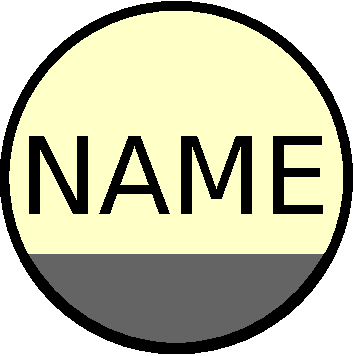
\includegraphics[scale = 0.3]{images/simpleCloneMarker}
  \caption{The \PD glyph for \glyph{simple clone marker} applied to a \glyph{simple chemical}}
  \label{fig:simpleCloneMarker}
\end{figure}

Unlike the \glyph{simple clone marker}, the \glyph{labeled clone marker} includes (unsurprisingly, given its name) an identifying label that can be used to identify equivalent clones elsewhere in the map.  This is particularly useful for stateful \glyph{EPNs}, because these can have a large number of state variables displayed and therefore may be difficult to visually identify as being identical. The filled area must be smaller than the unfilled one, but the be large enough to have a height larger than the \glyph{clone marker}'s label (cf below).

\begin{figure}[H]
  \centering
  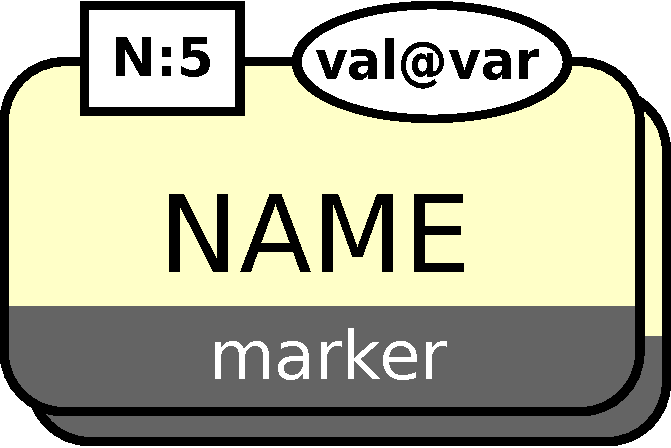
\includegraphics[scale = 0.3]{images/labeledCloneMarker}
  \caption{The \PD glyph for \glyph{labeled clone marker} applied to a \glyph{multimer} of  \glyph{macromolecules}.}
  \label{fig:labeledCloneMarker}
\end{figure}

